% IPSupport LLC -- quantization whitepaper.
% Build: tectonic whitepaper.tex   (figures: python make_figures.py)
% Every number in this document is taken from the projects' docs/FINDINGS.md
% and model cards in this repository; nothing is estimated.
\documentclass[10pt,letterpaper]{article}

\usepackage{fontspec}
\usepackage{unicode-math}
\setmainfont{Inter}[
  Path=fonts/, Extension=.otf,
  UprightFont=*-Regular, BoldFont=*-SemiBold,
  ItalicFont=*-Italic, BoldItalicFont=*-SemiBoldItalic]
\newfontfamily\interbold{Inter}[Path=fonts/, Extension=.otf, UprightFont=*-Bold]
\newfontfamily\interblack{Inter}[Path=fonts/, Extension=.otf, UprightFont=*-ExtraBold, WordSpace=1.9]
\setmonofont{lmmono10-regular.otf}
\setmathfont{latinmodern-math.otf}

\usepackage[letterpaper,margin=0.95in,top=1.0in,bottom=0.95in,headheight=14pt]{geometry}
\usepackage[table]{xcolor}
\usepackage{graphicx,booktabs,tabularx,array,colortbl,multirow}
\usepackage{enumitem,titlesec,fancyhdr,tikz,amsmath}
\usepackage[hidelinks]{hyperref}
\usepackage{caption}
\usepackage{float}
\usetikzlibrary{calc}

% ---- palette -------------------------------------------------------------
\definecolor{ink}{HTML}{14151A}
\definecolor{ink2}{HTML}{52514E}
\definecolor{paper}{HTML}{EEEDEA}
\definecolor{rule}{HTML}{D9D7D2}
\definecolor{brand}{HTML}{2A78D6}
\definecolor{brand2}{HTML}{6B4FD8}
\definecolor{thead}{HTML}{1F2027}
\definecolor{trow}{HTML}{F5F4F1}
\color{ink}

% ---- type & layout -------------------------------------------------------
\setlength{\parindent}{0pt}
\setlength{\parskip}{6pt}
\linespread{1.08}
\setlist{itemsep=2pt,topsep=2pt,leftmargin=1.2em}
\titleformat{\section}{\interbold\Large}{\thesection.}{0.5em}{}[{\color{rule}\titlerule[0.8pt]}]
\titleformat{\subsection}{\interbold\large}{\thesubsection}{0.6em}{}
\titleformat{\paragraph}[runin]{\interbold}{}{}{}[]
\titlespacing*{\section}{0pt}{14pt}{8pt}
\titlespacing*{\subsection}{0pt}{10pt}{4pt}
\captionsetup{font={small},labelfont={bf,color=brand},labelsep=period,justification=raggedright,singlelinecheck=false}
\captionsetup[table]{skip=4pt}

\newcommand{\hd}[1]{\textcolor{white}{\interbold #1}}
\newcommand{\best}[1]{\textbf{#1}}
\newcommand{\repo}[1]{\texttt{\small #1}}
\newcolumntype{L}{>{\raggedright\arraybackslash}X}
\renewcommand{\arraystretch}{1.18}

\pagestyle{fancy}
\fancyhf{}
\renewcommand{\headrulewidth}{0pt}
\fancyhead[L]{\interbold\small IPSupport\,\textcolor{brand}{LLC}}
\fancyhead[R]{\small\itshape\color{ink2}Any Model, Your Hardware, Your Data}
\fancyfoot[C]{\small\color{ink2}\thepage}

\hypersetup{pdftitle={Any Model, Your Hardware, Your Data},pdfauthor={IPSupport LLC}}

\begin{document}

% ======================================================================
% COVER
% ======================================================================
\thispagestyle{empty}
\begin{tikzpicture}[remember picture,overlay,every node/.style={execute at begin node={\hyphenpenalty=10000\exhyphenpenalty=10000}}]
  \fill[paper] (current page.north west) rectangle ($(current page.north east)+(0,-5.45in)$);
  \fill[ink]   ($(current page.north west)+(0,-5.55in)$) rectangle (current page.south east);
  \shade[left color=brand,right color=brand2]
     ($(current page.north west)+(0,-5.45in)$) rectangle ($(current page.north east)+(0,-5.55in)$);
  % faint diagonal hatching, like a quantization grid
  \begin{scope}
    \clip (current page.north west) rectangle ($(current page.north east)+(0,-5.45in)$);
    \foreach \i in {0,...,40} {
      \draw[rule,line width=0.4pt] ($(current page.north west)+(\i*0.32in-3in,-5.45in)$) -- ++(3.2in,3.2in);
    }
  \end{scope}
  \node[anchor=center] at ($(current page.north)+(0,-1.55in)$)
     {\interblack\fontsize{26}{28}\selectfont IPSupport\textcolor{brand}{\,LLC}};
  \node[anchor=center,text width=6.6in,align=center] at ($(current page.north)+(0,-3.0in)$)
     {\interblack\fontsize{34}{38}\selectfont Any\hspace{0.3em}Model.\\[2pt] Your\hspace{0.3em}Hardware.\hspace{0.3em}Your\hspace{0.3em}Data.};
  \node[anchor=center,text width=5.4in,align=center] at ($(current page.north)+(0,-4.35in)$)
     {\large\color{ink2}How we compress and fine-tune open models --- language, vision, speech, image and music --- to run on less hardware, faster, and on the client's own tasks. 23~open releases, every number reproducible.};
  % KPI row
  \foreach \x/\kbig/\ksub in {-2.25/{3.9×}/{less memory: Nemotron 30B\\at +2.5\% perplexity},0/{2.1×}/{faster full-duplex voice,\\20/20 answers right},2.25/{0}/{malformed tool calls after\\fine-tuning to our agent}} {
    \node[anchor=north,text width=2.1in,align=center,text=white] at ($(current page.north)+(\x in,-6.75in)$)
      {{\interbold\fontsize{26}{28}\selectfont \kbig}\\[6pt]{\small\color{rule}\ksub}};
  }
  \node[anchor=south,text=rule] at ($(current page.south)+(0,0.7in)$)
     {\small IPSupport LLC \quad·\quad October 2026 \quad·\quad ipsupport.us};
\end{tikzpicture}
\newpage

% ======================================================================
\tableofcontents
\clearpage

\section{Executive Summary}

IPSupport takes an open model and fits it to a client's hardware, speed target and data. We \textbf{compress} it, so it needs a fraction of the GPU memory and answers faster, and we \textbf{fine-tune} it on the client's own tasks and formats. Nothing in the method is tied to a model size: quantization and calibration run one layer at a time and resume from checkpoints, so the limit is disk and rented GPU-hours, not GPU memory. The largest checkpoints we have shipped so far are a 31B dense and a 30B mixture-of-experts model.

The savings are concrete. Gemma 4 31B goes from 62\,GB to 20.65\,GB and Nemotron 30B-A3B from 65.8\,GB to 16.7\,GB: a model that needed a data-center GPU runs on one consumer card or a laptop. Done naively, compression quietly costs the things users notice --- facts, code that compiles, a voice that answers on time. This paper shows how we avoid that, on 23 models we released openly.

Our toolkit has four parts, each validated on real checkpoints and real tasks:
\begin{itemize}
  \item \textbf{GPTQ, exact to the runtime.} Second-order error compensation~\cite{gptq}, with the quantization grid reproduced \emph{bit for bit} from the inference kernel, so the correction survives packing instead of being re-rounded away.
  \item \textbf{JANG: bits by component role.} On mixture-of-experts models we spend bits where they are cheap and sensitive (attention, shared experts) and save them on the 93\% of weights that are routed experts.
  \item \textbf{Riding the vendor's QAT.} When a vendor ships quantization-aware-trained weights, we transport them onto MLX \emph{losslessly} --- the same 4-bit codes as the vendor's own GGUF --- instead of re-quantizing them.
  \item \textbf{A $\Delta$KL-per-MB scan.} A greedy, measured choice of which few Linears earn 8 bits, under an explicit size budget.
\end{itemize}

Highlights, all published as open weights:
\begin{itemize}
  \item \textbf{Gemma 4 31B in 20.65\,GB} (from 62\,GB), KL 0.021 and 94.9\% top-1 agreement with the QAT master --- 8\,GB smaller than the community MLX build.
  \item \textbf{Gemma 4 12B at the same fidelity as the community QAT build with 3.1\,GB less}, 1.5× faster decode, now with vision and audio after we ported the model to our MLX fork.
  \item \textbf{A phone-sized Gemma 4 E2B GGUF built on Google's QAT}: Google's exact 4-bit codes plus a few scanned 8-bit Linears, 2.86\,GB at a PPL ratio of 0.986 to bf16 (Google's q4\_0: 3.35\,GB, 1.085).
  \item \textbf{Nemotron 3.5 Lightning 30B-A3B: PPL 5.24 in 16.7\,GB} (from 65.8\,GB), beating the third-party release whose bit map we reverse-engineered (5.43); bf16 is 5.11.
  \item \textbf{NemotronLabs VoiceChat 11B in real time on a base M5}: 185\,ms → 87.7\,ms per 80\,ms duplex frame, 20/20 answers right.
  \item \textbf{Fine-tuned to an agent's tools}: a LoRA taught Nemotron the tool names and call format of our coding agent IPSupport Code --- zero malformed tool calls in real sessions --- and the model was then quantized on the agent's own transcripts.
  \item \textbf{Diffusion and music}: GPTQ cuts velocity error 17--25\% at equal size on FLUX.2 klein and ACE-Step 1.5; Z-Image Turbo keeps its composition at 4~bits where plain rounding drifts.
\end{itemize}

Every claim here is backed by a script and a log in our public repository~\cite{repo}; Appendix~A lists all 23 releases.

% ======================================================================
\clearpage
\section{Portfolio at a Glance}

\begin{table}[H]
\centering\small
\caption{Model families we quantized and published. Sizes are weights on disk.}
\rowcolors{2}{trow}{white}
\begin{tabularx}{\linewidth}{>{\raggedright\arraybackslash}p{1.55in}>{\raggedright\arraybackslash}p{1.15in}L}
\rowcolor{thead}\hd{Family} & \hd{Formats} & \hd{Headline result}\\
Gemma 4 (E2B, E4B, 12B, 26B-A4B, 31B) & MLX, GGUF, MTP drafter & 31B in 20.65\,GB; 12B at community-QAT fidelity with 3.1\,GB less; phone E2B GGUF in 2.86\,GB on Google's QAT codes \\
Nemotron 3.5 Lightning 30B-A3B & MLX (+MTP head) & PPL 5.24 at 4.24\,bpw vs.\ bf16 5.11; self-speculative MTP preserved \\
Nemotron 3 Nano 4B & MLX & coding-agent LoRA (attention-only), 8-bit, 4.0\,GB from 7.5\,GB \\
NemotronLabs VoiceChat 11B & MLX & real-time duplex on a base M5 (87.7\,ms / 80\,ms frame) \\
FLUX.2 klein 4B & MLX (mflux) & GPTQ 4-bit: −17\% / −20\% velocity error vs.\ RTN, 5.3\,GB \\
Z-Image Turbo 6B & MLX (mflux) & GPTQ keeps 4-bit composition; mixed 8/4 best PSNR \\
ACE-Step 1.5 sft & MLX & GPTQ 4-bit: −25\% velocity error vs.\ RTN, singable lyrics \\
\end{tabularx}
\end{table}

All targets are \textbf{Apple Silicon} (MLX, via our forks of \repo{mlx-lm} and \repo{mlx-audio}) and \textbf{llama.cpp / ollama} (GGUF). Our MLX releases are built to run in \textbf{LLMTray}, our local AI runtime for macOS --- \emph{run local models, serve an OpenAI-compatible API, connect your coding agents and apps}.

% ======================================================================
\clearpage
\section{Methods}

\subsection{GPTQ: second-order error compensation}

For a linear layer with weights $W$ and calibration inputs $X$, post-training quantization seeks $\widehat W$ on the target grid minimizing the layer's output error $\lVert WX-\widehat W X\rVert_2^2$. The objective's Hessian is shared by every row,
\[
H = 2XX^{\top}.
\]
GPTQ~\cite{gptq} quantizes one column $q$ at a time and pushes its rounding error onto the columns not yet quantized, in proportion to the inverse Hessian:
\[
\delta = \frac{w_q-\operatorname{quant}(w_q)}{[H^{-1}]_{qq}},\qquad
w_{F}\;\leftarrow\; w_{F}-\delta\,[H^{-1}]_{F,q},
\]
with $F$ the remaining columns. A Cholesky factorization of $H^{-1}$ and lazy block updates make this a few GPU-minutes per layer. We calibrate on \emph{real} data for each modality --- text, COCO photographs, LibriSpeech audio, captured duplex conversations, and for diffusion models the activations of the model's own denoising loop.

Two engineering details mattered more than any hyperparameter:
\begin{itemize}
  \item \textbf{\texttt{cholesky\_solve}, not \texttt{cholesky\_inverse}.} The same inverse, ≈30× faster on a 2688-wide Hessian (0.7\,s vs.\ 24\,s). The slow call had silently inflated every GPTQ run.
  \item \textbf{Batched experts.} Same-shaped MoE experts are stacked into one $[E,\text{out},\text{in}]$ problem: 5.5× faster per block than a per-expert loop.
\end{itemize}

\subsection{Exactness: matching the runtime's grid bit for bit}

A GPTQ-corrected weight is only useful if the runtime stores exactly the code GPTQ chose. Our pipeline hands corrected weights to the stock MLX packer, which re-derives its own scales --- so any mismatch between GPTQ's grid and MLX's silently re-rounds the correction away. We measured three plausible formulas before reading the kernel: they scored PPL 27.68, 6{,}074{,}737 and 17.82 on a model whose naive rounding scores 6.54. MLX's actual affine grid, per group, with $n=2^{b}-1$:
\[
s=\pm\max\!\Big(\tfrac{w_{\max}-w_{\min}}{n},\,\varepsilon\Big),\quad
e=\begin{cases}w_{\min} & |w_{\min}|>|w_{\max}|\\ w_{\max} & \text{otherwise}\end{cases},\quad
q_0=\operatorname{round}(e/s),\quad s\leftarrow e/q_0,\quad \beta=e,
\]
\[
c=\operatorname{clamp}\big(\operatorname{round}((w-\beta)/s),\,0,\,n\big),\qquad \hat w=c\,s+\beta .
\]
Implemented once and verified bit-exact against \texttt{mx.quantize} before any pod time was spent; it is what lets 3-bit GPTQ beat 3-bit rounding (PPL 6.24 vs.\ 6.54) at identical size and speed.

\subsection{JANG: bits by component role}

A third-party release of Nemotron 30B-A3B (JANG\_2L-CRACK) beat our early mixes. Its \texttt{config.json} revealed why: bits assigned purely by \emph{component type}, not by layer depth. We adopted the map and ran it through our calibrated GPTQ instead of plain rounding:

\begin{table}[H]
\centering\small
\caption{The JANG component map (Nemotron 30B-A3B). Average 4.237 bits/weight.}
\rowcolors{2}{trow}{white}
\begin{tabular}{lcl}
\rowcolor{thead}\hd{Component} & \hd{Bits} & \hd{Why}\\
attention q/k/v/o & 8 & 6 of 52 layers; every token passes through \\
Mamba in/out projections & 6 & moderate share \\
MoE shared experts & 8 & one per block, always active \\
MoE routed up (\texttt{fc1}) / down (\texttt{fc2}) & 4 / 3 & 128 experts × 23 blocks, ≈93\% of weights \\
embeddings / lm\_head & 6 / 8 & --- \\
\end{tabular}
\end{table}

The lesson generalizes: \emph{bit allocation and calibration are independent, additive levers.} The same map plus our GPTQ scored PPL 5.24 against the original's 5.43. It also exposed a bug worth stating: the MLX port names routed experts \texttt{switch\_mlp.fc1/fc2}, not \texttt{up/down\_proj}, so two earlier ``mixed-precision'' releases (ours) had never upgraded the experts at all --- visible only in the packed tensor shapes on the Hub.

JANG is a MoE recipe. On dense models (Gemma E-series, VoiceChat's 9B) it degenerates to a mild 8/4 split with no structural win, and we say so in the results.

\subsection{Riding the vendor's QAT: lossless transport into MLX}

Google ships Gemma 4 quantization-aware-trained (QAT): a bf16 ``master'' and llama.cpp's q4\_0 of it. We checked that the GGUF \emph{is} q4\_0 of the master, bit for bit, and that the community MLX ports are \emph{not} on that grid (group 64, refit scales, MLPs at 8 bits). A q4\_0 block of 32 stores a scale $d$ and codes $c\in\{0,\dots,15\}$ with $w=d\,(c-8)$. MLX's affine 4-bit, group 32, computes $\hat w=s\,q+\beta$. Setting
\[
s=d,\qquad \beta=-8d
\]
makes the two grids identical; we pack Google's codes directly into MLX's words. The only deliberate loss is that MLX keeps scales in bf16, so each fp16 $d$ is rounded --- under $1/64$ of a step. Every 4-bit tensor's codes are checked against Google's GGUF: \textbf{275/275} (E2B), \textbf{342/342} (E4B), \textbf{328/328} (12B), \textbf{410/410} (31B) identical.

\subsection{Where the bits go: a \texorpdfstring{$\Delta$KL}{dKL}-per-MB scan}

Starting from the all-4-bit model, each candidate Linear $\ell$ is raised to 8 bits on its own and scored by the KL divergence it removes per megabyte it adds:
\[
g_\ell=\frac{\mathrm{KL}_{\text{base}}-\mathrm{KL}_{\text{base}+\ell}}{\Delta\mathrm{MB}_\ell},
\]
measured on 16 held-out windows against the bf16 master. Candidates are then taken greedily in descending $g_\ell$ under a budget $B$, and the chosen build is re-measured on 128 windows from disk. On E2B the build written to disk reproduces the scan's in-memory measurement to the second decimal (PPL 64.48 vs.\ 64.47). What earns the bits is not the large MLPs --- which the community build raises wholesale --- but about a hundred small, sensitive attention and per-layer projections.

\begin{figure}[H]
\centering
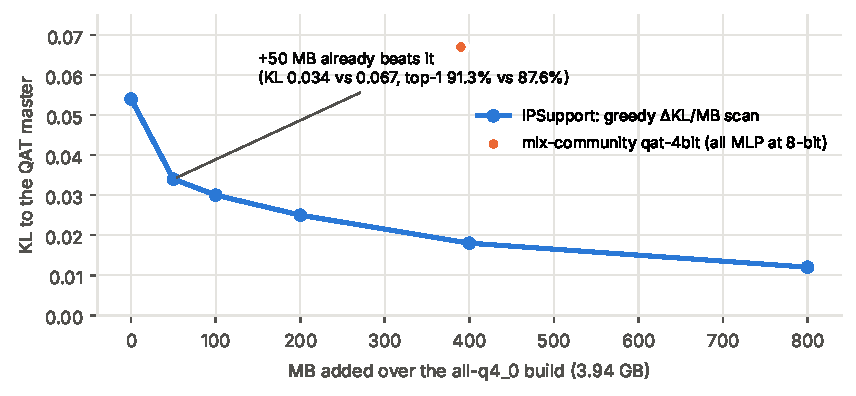
\includegraphics[width=\linewidth]{figures/fig_e2b_budget.pdf}
\caption{Gemma 4 E2B: KL to the QAT master vs.\ megabytes added by the greedy scan. Fifty megabytes, placed by the scan, beat a build that spends 390\,MB raising every MLP (128 windows × 512 tokens).}
\end{figure}

\subsection{Measuring what matters}

Perplexity alone misled us repeatedly, so every release is judged by the metric its users feel:
\begin{itemize}
  \item \textbf{Fidelity to the source:} KL divergence and top-1 agreement against the bf16 master, token by token. This is the honest measure of a quantization.
  \item \textbf{Capability:} code is \emph{compiled and run} (\texttt{g++ -std=c++20}, Python), not eyeballed; lyrics are transcribed by an independent Whisper; images are compared at a fixed seed.
  \item \textbf{The perplexity trap.} Gemma 4 checkpoints with \texttt{attention\_k\_eq\_v} (12B, 26B, 31B) score raw text in the thousands --- 2468 in llama.cpp, 2640 in transformers, 1786 in MLX for the 31B, on Google's own weights. They fall into attractor tokens and put 6--8\% of probability on control tokens. Scored as the model's \emph{reply} with the thinking channel closed, the 26B goes from 67{,}363 to 26.7. We publish chat-framed numbers for these models and say why.
\end{itemize}

% ======================================================================
\clearpage
\section{Results}

\subsection{Gemma 4}

\begin{figure}[H]
\centering
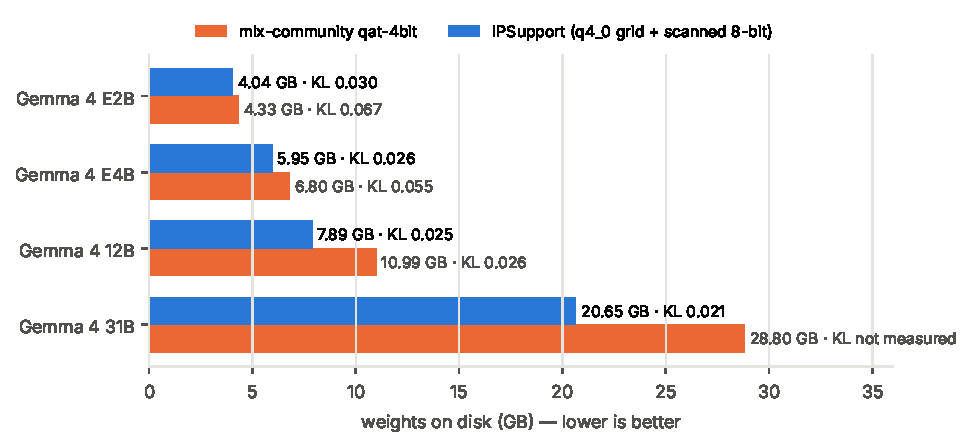
\includegraphics[width=\linewidth]{figures/fig_gemma_size.pdf}
\caption{Gemma 4 QAT builds: weights on disk, ours vs.\ \repo{mlx-community/gemma-4-*-it-qat-4bit}. KL is to the bf16 QAT master within each model (E2B/E4B raw-text windows, 12B/31B chat-framed); the community 31B was not measured.}
\end{figure}

\begin{table}[H]
\centering\small
\caption{Gemma 4 fidelity to the QAT master (128 windows × 512 tokens). Best in bold.}
\rowcolors{2}{trow}{white}
\begin{tabular}{llrrrr}
\rowcolor{thead}\hd{Model} & \hd{Build} & \hd{Size} & \hd{PPL} & \hd{KL} & \hd{Top-1}\\
E2B & \textbf{ours, q4\_0 grid + 126 Linears 8-bit} & \best{4.04\,GB} & \best{64.5} & \best{0.030} & \best{91.8\%}\\
 & mlx-community qat-4bit & 4.33\,GB & 66.2 & 0.067 & 87.6\%\\
 & mlx-community 4-bit RTN (no QAT) & 3.6\,GB & 239.7 & 0.853 & 66.3\%\\
E4B & \textbf{ours, q4\_0 grid} & \best{5.85\,GB} & \best{44.3} & \best{0.041} & \best{90.5\%}\\
 & mlx-community qat-4bit & 6.80\,GB & 45.4 & 0.055 & 89.0\%\\
12B$^{\dagger}$ & \textbf{ours, + 44 Linears 8-bit} & 7.89\,GB & \best{22.77} & \best{0.0253} & \best{93.44\%}\\
 & mlx-community qat-4bit & 10.99\,GB & 22.82 & 0.0259 & 93.35\%\\
 & mlx-community 4-bit (no QAT) & 6.74\,GB & 26.70 & 0.340 & 78.78\%\\
31B$^{\dagger}$ & \textbf{ours, + 35 Linears 8-bit} & 20.65\,GB & 27.82 & 0.0206 & 94.93\%\\
\end{tabular}

\smallskip
\footnotesize $^{\dagger}$Chat-framed windows (Section~3.6); master PPL 22.26 (12B) and 26.94 (31B). The published E4B adds 114 Linears at 8 bits (5.95\,GB, KL 0.026).
\end{table}

\paragraph{Speed on a base M5.} Fewer 8-bit tensors also mean less to read per token. E2B decodes at \textbf{67.5\,tok/s} vs.\ 54.7 for the community QAT build (+23\%); E4B at \textbf{34.9} vs.\ 26.0\,tok/s with 0.8\,GB less peak memory; 12B at \textbf{14.8} vs.\ 9.8\,tok/s (8.1 vs.\ 11.2\,GB peak). Plain 4-bit rounding is faster still on E2B (83.7\,tok/s) --- at four times the perplexity.

\paragraph{12B, now multimodal.} The 12B (\texttt{gemma4\_unified}) has no vision or audio towers: raw 48-pixel patches and 640-sample audio frames go through small embedders. Our MLX fork loaded it text-only; we ported both paths~\cite{fork}, fixed a cast that turned every pixel to zero once quantized, and matched mlx-vlm's features (cosine ≥ 0.9998). The 31B passes text and vision checks (23\,GB peak, measured on the A100); it needs a 48\,GB Mac (or a raised wired-memory limit).

\paragraph{E2B for phones.} Half of E2B's size is its per-layer embeddings. Dropping them from 6 to 4 bits costs almost nothing (KL $+0.0015$, ≈0.6\,GB saved); the scanned 8-bit Linears are kept because they halve KL. Google also ships a ``mobile'' QAT (int2/4/8 weights); we converted it exactly to MLX (2.57\,GB, 122.5\,tok/s) but it needs its int8 \emph{activations} --- without them PPL rises from 41 to 65 and the audio tower goes deaf --- so it suits an NPU runtime, not MLX or llama.cpp.

\begin{table}[H]
\centering\small
\caption{Gemma 4 E2B phone builds. GGUF: llama.cpp, 32 chunks of 512, against our bf16 GGUF of the master (PPL 42.84).}
\rowcolors{2}{trow}{white}
\begin{tabular}{lrrrr}
\rowcolor{thead}\hd{Build} & \hd{Size} & \hd{PPL} & \hd{vs.\ bf16} & \hd{Decode (M5)}\\
\textbf{ours, GGUF} (Q4\_0 + PLE Q4\_K + Q8\_0 Linears) & \best{2.86\,GB} & \best{42.24} & \best{×0.986} & --- \\
Google \repo{gemma-4-E2B\_q4\_0-it.gguf} & 3.35\,GB & 46.47 & ×1.085 & --- \\
\textbf{ours, MLX} (PLE 4-bit, towers 4-bit) & 3.10\,GB & 36.44$^{\ddagger}$ & --- & 70.2\,tok/s \\
\end{tabular}

\smallskip
\footnotesize $^{\ddagger}$128 chat windows, master 36.04; KL 0.0242, top-1 92.48\%. All 149 of our Q4\_0 tensors are byte-identical to Google's; the gain is the Q8\_0 Linears.
\end{table}

\paragraph{26B-A4B (MoE): GPTQ JANG, GGUF and a speculative drafter.} The 128-expert 26B is quantized with per-expert GPTQ (calibration rows bucketed by the real routing, all 128 experts solved in one batch), attention at 8 bits, experts at 4, routers untouched: \textbf{15\,GB from 51.6\,GB}. The GGUF build (imatrix on a broad corpus, attention Q5\_K, experts IQ3\_S) is 12.5\,GB. Google's 4-layer MTP drafter had no MLX support; we implemented it~\cite{fork} and published it at 8 bits (446\,MB): \textbf{35.8\,→\,52.9\,tok/s} on a short prompt, 32.7\,→\,41.7 at 3.9k context, with the main model's output unchanged.

\subsection{Nemotron 3.5 Lightning 30B-A3B and Nemotron 3 Nano 4B}

\begin{figure}[tb]
\centering
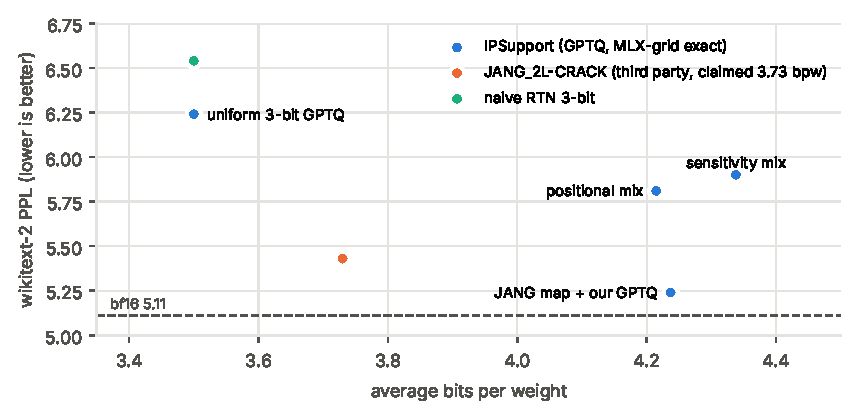
\includegraphics[width=\linewidth]{figures/fig_nemotron_ppl.pdf}
\caption{Nemotron 3.5 Lightning 30B-A3B, wikitext-2 perplexity vs.\ bits per weight (20 × 512 tokens). The JANG component map run through our grid-exact GPTQ lands closest to bf16.}
\end{figure}

\begin{table}[H]
\centering\small
\caption{Nemotron 30B-A3B (hybrid Mamba-2 / attention / 128-expert MoE, 52 layers). The PPL column relative to bf16 is the one to read: uniform 3-bit is an extreme quant.}
\rowcolors{2}{trow}{white}
\begin{tabular}{lrrrr}
\rowcolor{thead}\hd{Build} & \hd{PPL} & \hd{vs.\ bf16} & \hd{Size} & \hd{bits/weight}\\
bf16 (reference) & 5.11 & --- & 65.8\,GB & 16\\
\textbf{JANG map + our GPTQ (recommended)} & \best{5.24} & \best{+2.5\%} & \best{16.7\,GB} & 4.237\\
JANG\_2L-CRACK (third party, presumed RTN) & 5.43 & +6.3\% & 16\,GB & ≈3.73 (their label)\\
uniform 3-bit, our GPTQ (extreme) & 6.24 & +22\% & 13.8\,GB & 3.5\\
uniform 3-bit, naive rounding (extreme) & 6.54 & +28\% & 13\,GB & 3.5\\
\end{tabular}
\end{table}

\paragraph{Speed is set by the bit map's structure, not its average.} Uniform 3-bit decodes at 65--69\,tok/s; both JANG builds, ours and the third party's, at 42--43\,tok/s despite different calibration and average bits. JANG spends its bits on the dense components that every token touches, so ``cheap on disk'' and ``cheap per token'' are opposite properties on this architecture. But speed is the only thing uniform 3-bit wins: it is an \textbf{extreme quant}, +22\% perplexity over bf16 against JANG's +2.5\%, and in real use its answers degrade markedly. We keep it on the Hub as the latency end of the frontier and recommend the JANG build for anything that has to be right.

\paragraph{Why a LoRA: our agent's tools.} Both Nemotrons carry a LoRA for \textbf{IPSupport Code}, our local coding agent, and it exists to fix one concrete failure: driving the agent, the base model kept getting our tools wrong --- wrong tool names, wrong parameter names, malformed JSON in the call. We trained on the real sessions where it failed, plus synthetic conversations covering the same patterns, merged the adapter into bf16, and only then quantized, calibrating GPTQ on the agent's own tool-call transcripts. Result in real use: \textbf{zero malformed tool calls across a session}, and on held-out tool-call data PPL 2.464 → 2.379 (−3.5\%) for +0.8\% on generic prose --- the intended trade for a model that lives inside an agent.

\paragraph{\dots and what it taught us.} Two findings came only from running the code the model wrote: training attention and MLP adapters \emph{together} on the 4B dropped C++ compile-and-run from 6/9 to 0/9 at any rank or length, while either half alone matched the base --- so the shipped 4B adapter is attention-only. And GPTQ, calibrated on text with no C++ in it, scored 2/9 where plain 8-bit rounding scored 4/9 (bf16: 6/9): calibration preserves what the calibration set contains, so the 4B ships with the method that won. The fine-tune also leaves a reflex: given tools in a plain chat, the 30B reaches for one on a greeting 10 times in 20 (the base: 0). Right for an agent, wrong for small talk; LLMTray sends a system rule that cuts it on questions from 14/20 to 4--6/20, and the cards say so.

\paragraph{Keeping the MTP head.} The 30B ships a 1.34B-parameter multi-token-prediction head that every public quant had silently dropped: transformers discards \texttt{mtp.*} on load, before any merge or quantization runs. We extract it from the untouched checkpoint and splice it back into the finished MLX model; self-speculative decoding is bit-exact against greedy. Along the way we fixed two decoding bugs in the MTP path~\cite{fork}: a fused single-step SSM kernel that corrupted the Mamba state on every rejected draft, and an unchunked prefill that made 400-token prompts run out of memory (now flat at 18.4\,GB up to 4000 tokens).

\subsection{NemotronLabs VoiceChat 11B: real-time duplex on a laptop}

VoiceChat is a full duplex voice model: a streaming FastConformer encoder, the Nemotron Nano 9B hybrid LLM, a T5Gemma TTS and a 22\,kHz codec. It must produce one 80\,ms audio frame in under 80\,ms on a base M5 --- fanless, 19\,GB GPU budget.

\begin{figure}[H]
\centering
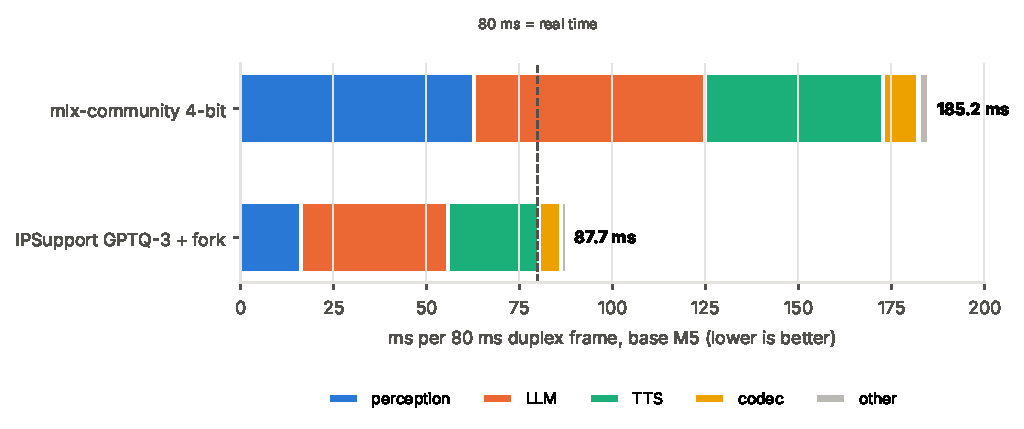
\includegraphics[width=\linewidth]{figures/fig_voicechat_latency.pdf}
\caption{Milliseconds per 80\,ms frame, 20 spoken questions, idle base M5. Baseline: the community 4-bit checkpoint. Ours: GPTQ 3-bit LLM plus runtime fixes in our \repo{mlx-audio} fork.}
\end{figure}

GPTQ 3-bit on the LLM, calibrated on 256 captured real conversations, answered \textbf{20/20} questions with a reply word-error rate of 0.043, the lowest among the variants that answered every question. The rest came from the runtime: perception was running in float32 because mel frames arrived that way (51\,→\,17\,ms after the cast; 13.6\,ms compiled), and the TTS head computed every mixture component instead of the sampled one. The LLM now sits at the memory-bandwidth floor (≈105\,GB/s effective). A second release adds 8-bit speech towers (6.43\,GB, 83.3\,ms cold), and pausing the TTS while the model listens brings an average frame to 69.1\,ms (real-time factor 0.86). We tried a 2-bit MLP: 4\,ms faster, wrong answers (``blue + yellow = gray''). It was not shipped.

\subsection{Diffusion and audio models}

For diffusion models the calibration signal is the model's own sampling: we hook every target Linear through real denoising steps and sum each Hessian over every token of every step.

\begin{table}[H]
\centering\small
\caption{GPTQ vs.\ plain rounding (RTN) at equal size. Velocity error is teacher-forced $\lVert v_q-v_{\text{bf16}}\rVert/\lVert v_{\text{bf16}}\rVert$, so trajectory drift does not compound into it.}
\rowcolors{2}{trow}{white}
\begin{tabularx}{\linewidth}{>{\raggedright\arraybackslash}p{1.35in}lL}
\rowcolor{thead}\hd{Model} & \hd{Build} & \hd{GPTQ vs.\ RTN}\\
FLUX.2 klein 4B & 4-bit, 5.3\,GB & velocity error 0.202 vs.\ 0.244 (−17\%) text-to-image, 0.136 vs.\ 0.171 (−20\%) edit; lower on all 9 held-out samples; PSNR 19.6 vs.\ 18.7\,dB\\
ACE-Step 1.5 sft (music) & 4-bit DiT, 1.65\,GB & velocity error 10.4\% vs.\ 13.9\% (−25\%), condition encoder 2.7\% vs.\ 5.0\% (−47\%)\\
Z-Image Turbo 6B & 4-bit / mixed 8+4 & PSNR 17.1 vs.\ 16.6\,dB; at 4 bits RTN shifts the whole composition, GPTQ holds it; attention-8 / FFN-4 reaches 17.4\,dB for +0.8\,GB\\
\end{tabularx}
\end{table}

\paragraph{FLUX.2 klein.} The text encoder is stock Qwen3-4B, byte for byte, and the pipeline only reads hidden states 9, 18 and 27 --- so layers 27--35 never touch the image. We drop them: prompt embeddings stay bit-identical and 1\,GB disappears. With the encoder at 8 bits and the transformer at GPTQ 4 bits, the model generates and edits in 5.3\,GB (bf16: 16\,GB), 7.3\,GB peak at 1024\textsuperscript{2}.

\paragraph{ACE-Step.} Run through the stock MLX audio stack, the sft model sang gibberish. Two causes, both measured with an independent Whisper: the planner's audio hints break the sft DiT, and the classifier-free-guidance branch encoded zeros instead of the trained null embedding. Fixed, it sings intelligibly: word-error rate 0.22 in bf16, 0.24 at 8 bits, 0.29 with GPTQ 4-bit, peak memory 10.6\,/\,8.6\,/\,7.5\,GB.

% ======================================================================
\section{Engineering We Fixed Upstream}

Quantization work runs into the runtime. These fixes are merged in our forks or published as patches:
\begin{itemize}
  \item \textbf{Gemma 4 KV-shared layers crashed with a quantized KV cache} (a shared layer handed a quantized tuple to the unquantized attention path) --- a production crash in LLMTray.
  \item \textbf{Gemma 4 MTP drafter for MLX}, with an exact cache rollback past the 1024-token sliding window, and a RoPE offset bug that made the drafter useless whenever the server reused a cached prefix (+48\% offline, nothing in the app until fixed).
  \item \textbf{Nemotron-H MTP}: the speculative step left the cache one token short, dropping the last token of every assistant reply from multi-turn context; plus the SSM rollback and prefill-memory fixes above.
  \item \textbf{Gemma 4 GGUF that chats correctly}: a tokenizer conversion crash, control tokens tagged as text (they leaked \texttt{<|channel>thought} into replies), and an ollama \texttt{RENDERER}/\texttt{PARSER} Modelfile that a Hub repo cannot express on its own.
  \item \textbf{Three llama.cpp bugs mistagging dense Nemotron-H as MoE} after a \texttt{save\_pretrained} round trip; conversion ``succeeded'' and the file would not load.
  \item \textbf{\texttt{gemma4\_unified} vision and audio} in MLX (Section~4.1).
\end{itemize}

% ======================================================================
\enlargethispage{3\baselineskip}
\section{Limitations and Lessons}

We publish our negative results too; several shaped the methods above.
\begin{itemize}
  \item \textbf{QAT beats post-training quantization.} Where a vendor ships QAT weights we transport them rather than re-quantize; our own PTQ of the non-QAT E2B was not released.
  \item \textbf{Calibration preserves what it sees.} GPTQ helps on the calibration distribution and can cost capabilities outside it (Section~4.2). We calibrate per modality and verify with task tests.
  \item \textbf{Perplexity is not a quality measure on its own.} It missed a broken \texttt{<think>} close, a C++ regression, and it reports thousands for healthy Gemma 4 models.
  \item \textbf{2 bits cost facts.} On VoiceChat's LLM every 2-bit MLP variant answered questions wrong that 3 bits answered right.
  \item \textbf{Laptops throttle.} On a fanless M5 the same build measured 84\,ms and then 117\,ms in back-to-back runs. Our timings come from cool, idle machines in alternated order, and real long sessions will run slower than the cold figures.
  \item \textbf{Raw sizes are not everything.} The 31B at 20.65\,GB still exceeds a 32\,GB Mac's GPU budget once the KV cache grows; we state memory requirements on every card.
\end{itemize}

% ======================================================================
\clearpage
\appendix
\section{All Releases}

\begin{table}[H]
\centering\footnotesize
\caption{Public releases on Hugging Face (\repo{roman220220/\dots}). Sizes are weights; downloads are the Hub's 30-day count at the time of writing (3{,}000+ in total).}
\rowcolors{2}{trow}{white}
\begin{tabularx}{\linewidth}{>{\raggedright\arraybackslash}p{2.95in}lL}
\rowcolor{thead}\hd{Repository} & \hd{Format} & \hd{Contents}\\
gemma-4-31B-it-qat-mlx & MLX & 20.65\,GB, text + vision\\
gemma-4-12B-it-qat-mlx & MLX & 7.89\,GB, text + vision + audio\\
gemma-4-E4B-it-qat-mlx & MLX & 5.95\,GB, text + vision + audio\\
gemma-4-E2B-it-qat-mlx & MLX & 4.04\,GB, text + vision + audio\\
gemma-4-E2B-it-qat-phone-mlx & MLX & 3.10\,GB, phone build\\
gemma-4-E2B-it-qat-phone-GGUF & GGUF & 2.86\,GB + Google's mmproj\\
gemma-4-26B-A4B-it-gptq-mlx-jang & MLX & ≈15\,GB, MoE, text + vision\\
gemma-4-26B-A4B-it-GGUF-jang-imatrix & GGUF & 12.5\,GB + mmproj + MTP drafter\\
gemma-4-26B-A4B-it-assistant-mlx-8bit & MLX & 446\,MB MTP drafter\\
Nemotron-3.5-Lightning-30B-A3B-JANG-GPTQ-ipsupport-code-lora-MTP & MLX & coding-agent LoRA + MTP head\\
Nemotron-3.5-Lightning-30B-A3B-JANG-GPTQ-ipsupport-code-lora & MLX & coding-agent LoRA\\
nemotron-30b-a3b-gptq-jang-component & MLX & 16.7\,GB, JANG + GPTQ, 4.237\,bpw\\
nemotron-30b-a3b-gptq3bit-g64 & MLX & uniform 3-bit GPTQ, 13.8\,GB\\
NVIDIA-Nemotron-3-Nano-4B-JANG-GPTQ-ipsupport-code-lora & MLX & coding-agent LoRA, 8-bit\\
NemotronLabs-VoiceChat-11B-gptq-mlx-3bit & MLX & real-time duplex voice\\
NemotronLabs-VoiceChat-11B-gptq-mlx-mixed & MLX & + 8-bit speech towers, 6.43\,GB\\
flux2-klein-4b-mlx-mixed & MLX & generate + edit, 5.3\,GB\\
z-image-turbo-gptq-mlx-4bit & MLX & 5.5\,GB\\
z-image-turbo-gptq-mlx-8bit & MLX & ≈10\,GB\\
z-image-turbo-gptq-mlx-mixed & MLX & attention 8 / FFN 4, 6.3\,GB\\
ACE-Step1.5-sft-MLX-bf16 & MLX & reference\\
ACE-Step1.5-sft-MLX-8bit & MLX & 8-bit DiT\\
ACE-Step1.5-sft-MLX-gptq-4bit & MLX & GPTQ 4-bit DiT\\
\end{tabularx}
\end{table}

\section{Evaluation Protocols}

\begin{itemize}
  \item \textbf{Language models:} wikitext-2 test, BOS at the start of every window (Gemma needs it); KL and top-1 agreement against the bf16 source checkpoint over 128 windows of 512 tokens. Chat-only checkpoints are scored as the assistant's reply with the thinking channel closed.
  \item \textbf{Code:} 3 seeds × 3 temperatures per prompt, the extracted code compiled with \texttt{g++ -std=c++20} or executed in Python; pass/fail counted.
  \item \textbf{Speech:} 20 spoken questions; keyword accuracy and reply word-error rate from an independent Whisper; per-frame timings on an idle base M5 after a 5-minute cool-down, order alternated.
  \item \textbf{Music:} 3 songs × 4 seeds, 30\,s each, Whisper word-error rate against the requested lyrics.
  \item \textbf{Images:} fixed seeds, PSNR against bf16 and teacher-forced velocity error on held-out prompts and edits.
\end{itemize}

\clearpage
\section{Reproducibility}

{\raggedright
Every release is produced by a resumable pipeline in our repository~\cite{repo} --- \texttt{qat\_mlx\_pipeline.sh} (Gemma QAT), \texttt{gemma4\_mlx\_pipeline.sh} and \texttt{gemma4\_26b\_gguf\_pipeline.sh} (GPTQ JANG and GGUF), \texttt{run\_pipeline.sh} (Nemotron) --- with calibration on a rented A100 and conversion checked on a Mac. Each project's \texttt{docs/FINDINGS.md} records every measurement, including the ones that went wrong.\par}

{\raggedright
\begin{thebibliography}{9}
\bibitem{gptq} E.~Frantar, S.~Ashkboos, T.~Hoefler, D.~Alistarh. \emph{GPTQ: Accurate Post-Training Quantization for Generative Pre-trained Transformers.} ICLR 2023.
\bibitem{repo} IPSupport LLC. \emph{quant-ternary: quantization pipelines and findings.} \url{https://github.com/rromenskyi/quant-ternary}
\bibitem{fork} IPSupport LLC. \emph{mlx-lm fork with Gemma 4 and Nemotron-H support.} \url{https://github.com/ipsupport-llc/mlx-lm}
\end{thebibliography}
}

% ======================================================================
% BACK COVER
% ======================================================================
\newpage
\thispagestyle{empty}
\begin{tikzpicture}[remember picture,overlay]
  \fill[ink] (current page.north west) rectangle (current page.south east);
  \shade[left color=brand,right color=brand2]
     ($(current page.south west)+(0,2.6in)$) rectangle ($(current page.south east)+(0,2.68in)$);
  \node[anchor=center,text=white] at ($(current page.center)+(0,1.2in)$)
     {\interblack\fontsize{24}{26}\selectfont IPSupport\textcolor{brand}{\,LLC}};
  \node[anchor=center,text width=5in,align=center,text=rule] at ($(current page.center)+(0,0.35in)$)
     {\large Senior engineering for cloud, voice and AI systems.};
  \node[anchor=center,text width=5in,align=center,text=white] at ($(current page.center)+(0,-0.85in)$)
     {7533 S Center View Ct \#6055\\ West Jordan, UT 84084, USA\\[8pt]
      +1 (385) 297-0034\\ hello@ipsupport.us\\[8pt]
      {\interbold ipsupport.us}};
  \node[anchor=center,text width=5.4in,align=center,text=rule] at ($(current page.south)+(0,1.6in)$)
     {\small LLMTray --- Local AI Runtime for macOS: run local models, serve an OpenAI-compatible API, connect your coding agents and apps.\\[4pt] IPSupport Code --- your AI coding agent for real repositories.};
\end{tikzpicture}

\end{document}
